%%%%%%%%%%%%%%%%%%%%%%%%%%%%%%%%%%%%%%%%%%%%%%%%%%%%%%%%%%%%%%%%%%%%%%%%%%%%%%%%
% Memoria para trabajos y entregas de laboratorio de la Escuela Superior de    %
% Informática (ESI) de Ciudad Real, UCLM.                                      %
%   Versión: Octubre - 2018                                                    %
%   Desarrollada por José Ángel Martín Baos                                    %
%                                                                              %
% Recursos:			                                                           %
%   - Contenidos del curso “LaTeX esencial para preparación de Trabajo Fin de  %
%     Grado, Tesis y otros documentos académicos” impartido por el profesor    %
%     Jesús Salido.                                                            %
%                                                                              %
% Disponible en: https://github.com/JoseAngelMartinB/PlantillaTrabajosLaTeX    %
%%%%%%%%%%%%%%%%%%%%%%%%%%%%%%%%%%%%%%%%%%%%%%%%%%%%%%%%%%%%%%%%%%%%%%%%%%%%%%%%

\documentclass[11pt]{article}

% PAQUETES USADOS:
\usepackage{natbib}
\usepackage{url}
\usepackage[utf8]{inputenc} % Codificación (Permite carácteres españoles)
\usepackage{amsmath}
\usepackage{graphicx}
\graphicspath{{images/}} % Carpeta en la cual se van a buscar las imagenes
\usepackage{subfigure}	% Permite la Inclusión de subfiguras
%\usepackage{parskip} % Suprime la identación de los parrafos.
\setlength{\parskip}{3mm} % Longitud del espaciado entre parrafos
\usepackage[hidelinks]{hyperref} % Referencias (links)
\usepackage{fancyhdr}
\usepackage{vmargin}
\usepackage{paralist} % Permite un mayor control sobre las listas
\usepackage{textcomp,marvosym,pifont} % Generación de símbolos especiales
\usepackage[usenames,dvipsnames,svgnames,x11names,table]{xcolor}
\usepackage{enumerate}

% CONFIGURACIÓN DE LA PÁGINA:
\setpapersize{A4} % Formato del papel - A4
\setmarginsrb{3 cm}{2.5 cm}{3 cm}{2.5 cm}{1 cm}{1.5 cm}{1 cm}{1.5 cm} % Margenes

% Complemento para insertar código en la memoria:
%   Basado en 'Listados de código cómodos y resultones con listings'
%   de David Villa en http://crysol.org/es/node/909
\usepackage{color}
\definecolor{gray97}{gray}{.97}
\definecolor{gray75}{gray}{.75}
\definecolor{gray45}{gray}{.45}
\usepackage{listings}
\lstset{ frame=Ltb,
	framerule=0pt,
	aboveskip=0.5cm,
	framextopmargin=3pt,
	framexbottommargin=3pt,
	framexleftmargin=0.4cm,
	framesep=0pt,
	rulesep=.4pt,
	backgroundcolor=\color{gray97},
	rulesepcolor=\color{black},
	texcl=true,
	%
	stringstyle=\ttfamily,
	showstringspaces = false,
	basicstyle=\small\ttfamily,
	commentstyle=\color{gray45},
	keywordstyle=\bfseries,
	%
	numbers=left,
	numbersep=15pt,
	numberstyle=\tiny,
	numberfirstline = false,
	breaklines=true,
}
% Minimizar fragmentado de listados
\lstnewenvironment{listing}[1][]
{\lstset{#1}\pagebreak[0]}{\pagebreak[0]}

\lstdefinestyle{consola}
{basicstyle=\scriptsize\bf\ttfamily,
	backgroundcolor=\color{gray75},
}

\lstdefinestyle{C}
{language=C,
}

%OTROS PAQUETES:
\usepackage{float} % Permite usar H en las figuras, de manera que se coloquen en la posición exacta en la que están en el código.

% Añade un comando para crear indicaciones de pulsación de teclas
\usepackage{tikz} % Paquete especializado en gráficos
\usetikzlibrary{shadows} % Necesario para poder crear nuevo comando de indicación de pulsación de tecla.
\newcommand*\tecla[1]{%
	\tikz[baseline=(key.base)]
	\node[%
	draw,
	fill=white,
	drop shadow={shadow xshift=0.25ex,shadow yshift=-0.25ex,fill=black,opacity=0.75},
	rectangle,
	rounded corners=2pt,
	inner sep=1pt,
	line width=0.5pt,
	font=\scriptsize\sffamily
	](key) {#1\strut}
	;
}

\newif\ifspanish % Condicional que permite seleccionar el lenguage.
\newif\ifmultipleauthors % Condicional que permite multiples autores
\spanishtrue
\multipleauthorsfalse


%%%%%%%%%%%%%%%%%%%%%%%%%%%%%%%%%%%%%%%%%%%%%%%%%%%%%%%%%%%%%%%%%%%%%%%%%%%%%%%%
%%%%%%%%%				Principales variables del documento			   %%%%%%%%%

\title{Práctica 2: Renderizado Gráfico}							% Titulo
\author{David Camuñas Sánchez}							% Autor

\date{29 de abril de 2020}											% Fecha
\newcommand{\subject}{Diseño de Infraestructuras de Red}						% Asignatura
\newcommand{\course}{Grado en Ingeniería Informática}	% Curso
%\newcommand{\course}{Máster Universitario en Ingeniería Informática}	% Curso
\newcommand{\courseyear}{2019 - 2020} 					% Curso académico
%\spanishfalse	    	% Descomentar esta línea si el trabajo está en inglés
%\multipleauthorstrue   % Descomentar esta línea si hay varios autores

%%%%%%%%%%%%%%%%%%%%%%%%%%%%%%%%%%%%%%%%%%%%%%%%%%%%%%%%%%%%%%%%%%%%%%%%%%%%%%%%

\ifspanish
	\usepackage[spanish]{babel} % Paquete de español
	\newcommand{\dateText}{Fecha:}
	\renewcommand{\lstlistingname}{Listado} % Renombrar listados para que aparezcan en español.
	% Algoritmos
	\usepackage[ruled,vlined,spanish]{algorithm2e} % Permite pseudocódigos. NECESARIO INSTALAR texlive-science (sudo apt-get install texlive-science)
\else
	\usepackage[english]{babel} % Paquete de inglés
	\newcommand{\dateText}{Date:}
	% Algoritmos
	\usepackage[ruled,vlined,english]{algorithm2e}
\fi

\makeatletter
\let\thetitle\@title
\let\theauthor\@author
\let\thedate\@date
\makeatother

% Formato de página:
\pagestyle{fancy}		% Formato por defecto - Recomendado
%\pagestyle{headings} 	% Formato para libros
\fancyhf{}
\ifmultipleauthors
	\chead{\thetitle}
\else
	\rhead{\subject}
	\lhead{\thetitle}
\fi
\cfoot{\thepage}

\begin{document}

%%%%%%%%%%%%%%%%%%%%%%%%%%%%%%%%%%%%%%%%%%%%%%%%%%%%%%%%%%%%%%%%%%%%%%%%%%%%%%%%
%%%%%%%%							Portada							   %%%%%%%%%

\begin{titlepage}
	\centering
	\begin{minipage}[t]{\textwidth}
		\raisebox{-0.5\height}{
\includegraphics[scale = 0.5]{uclm.jpg}} 	% Logo de la universidad
		\hspace{\fill}
		\raisebox{-0.5\height}{
\includegraphics[scale = 0.5]{open-mpi.png}} 	% Logo de open-mpi
	\end{minipage}
	\\[2.25 cm]
    \textsc{\LARGE Universidad de Castilla-La Mancha}\\[1 cm]	% Nombre de la universidad
    \textsc{\LARGE Escuela Superior de Informática}\\[2.0 cm]
	\textsc{\Large \subject}\\[0.5 cm]				% Asignatura
	\textsc{\large \course \\ \courseyear}\\[2 cm]				% Curso
	\rule{\linewidth}{0.2 mm} \\[0.4 cm]
	{ \huge \bfseries \thetitle}\\
	\rule{\linewidth}{0.2 mm} \\[2.5 cm]

	\vspace*{\fill}
	\begin{minipage}{0.4\textwidth}
		\begin{flushleft} \large
			\ifspanish
				\ifmultipleauthors
					\emph{Autores:}\\
				\else
					\emph{Autor:}\\
				\fi
			\else
				\ifmultipleauthors
					\emph{Authors:}\\
				\else
					\emph{Author:}\\
				\fi
			\fi
			\theauthor
			\end{flushleft}
			\end{minipage}~
			\begin{minipage}{0.4\textwidth}
			\begin{flushright} \large
			\emph{\dateText} \\
			\thedate
		\end{flushright}
	\end{minipage}\\[2.25 cm]


\end{titlepage}

%%%%%%%%%%%%%%%%%%%%%%%%%%%%%%%%%%%%%%%%%%%%%%%%%%%%%%%%%%%%%%%%%%%%%%%%%%%%%%%%
%%%%%%%%%						   	Índice					      	   %%%%%%%%%

\tableofcontents
\pagebreak


%%%%%%%%%%%%%%%%%%%%%%%%%%%%%%%%%%%%%%%%%%%%%%%%%%%%%%%%%%%%%%%%%%%%%%%%%%%%%%%%
%%%%%%%%%							Documento						   %%%%%%%%%
\section{Enunciado}
Utilizaremos las primitivas pertinentes \textbf{\textit{MPI2}} como acceso paralelo a disco y
gestión de procesos dinámico:\\
Inicialmente el usuario lanzará un solo proceso mediante \textit{mpirun -np 1
./pract2}. Con ello MPI lanza un primer proceso que será el que tiene acceso a
la pantalla de gráficos pero no a disco. Él mismo será el encargado de levantar
N procesos (con N definido en tiempo de compilación como una constante) que
tendrán acceso a disco pero no a gráficos directamente.

Los nuevos procesos lanzados se encargarán de leer de forma paralela
los datos del archivo foto.dat. Después, se encargarán de ir enviando los pixels
al primer elemento de proceso para que éste se encargue de representarlo en
pantalla.

Usaremos la plantilla pract2.c para comenzar a desarrollar la práctica.
En ella debemos completar el código que ejecuta el proceso con acceso a la
ventana de gráficos (rank 0 inicial) y la de los procesos “trabajadores”.
Se proporciona el archivo foto.dat. La estructura interna de este archivo
es 400 filas por 400 columnas de puntos.\\
Cada punto está formado por una
tripleta de tres “unsigned char” correspondiendo al valor R,G y B de cada uno
de los colores primarios. Estos valores se pueden usar para la función
\textit{dibujaPunto}().

\newpage
% Sección: Intruducción
\section{Introducción}
El objetivo de esta práctica es la creación de un programa de rendrerizado gráfico, mediante el uso de las \textit{funciones} que nos ofrece \textbf{\textit{MPI}}.

A la hora de analizar una imagen, en este caso foto.dat, se puede tratar como si fuese una matriz de \textit{X} (filas) por \textit{Y} (columnas) dimensiones. En este caso, se trata de una matriz cuadrada de \textit{400 píxeles}, es decir, donde tanto el valor de las \textbf{filas} y \textbf{columnas} es de \textbf{400}. Por tanto el número total de pixeles que forman la matriz, es \textbf{$400^2$} \textit{($L^2$)} = \textbf{160000 píxeles}.\\
Estos valores estan indicados en el programa, en forma de constantes, en concreto, en el archivo \textit{include/definitions.h}.\\

En la Figura \ref{fig:intro}, se puede observar la estructura de una imagen junto con la imagen a renderizar. Donde cada píxel está formado por una
tripleta de tres parámetros de tipo “\textit{unsigned char}” correspondiendo al valor R,G y B de cada uno de los \textit{colores primarios}.

\begin{figure}[H]
  \centering
  \subfigure[Pixeles de una imagen]{
    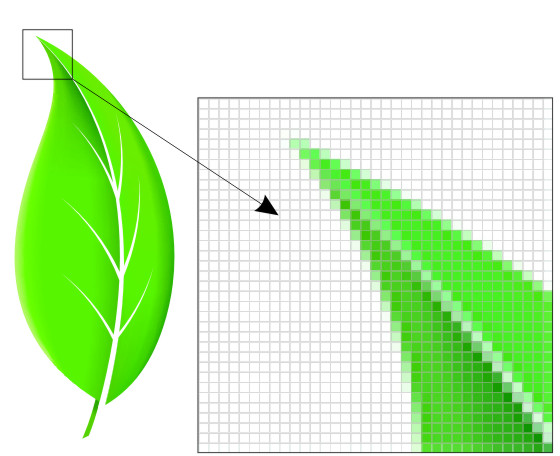
\includegraphics[width=70mm]{pixeles.jpg}
  }
  \subfigure[Imagen a renderizar]{
  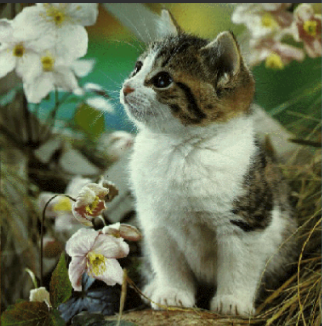
\includegraphics[width=50mm]{cat.png}
  
  }
  \caption{Representación de píxeles que forman una imagen}
  \label{fig:intro}
\end{figure}

\clearpage


\section{Planteamiento de la solución}
El programa comienza con a creación de un solo proceso, este proceso es el proceso principal, el cual corresponde al proceso cuyo \textit{RANK} es igual a 0. También conocido a lo largo del programa como el proceso \textbf{\textit{maestro}}.\\
Una vez lanzado el proceso \textit{maestro}, este creará una ventana gráfica haciendo uso de la librería \textit{\textbf{lX11}} (función \textit{initX()}). Además también creará \textbf{N} procesos hijos, conocidos a lo largo del programa como \textit{\textbf{esclavos o trabajadores}} (definidos con la constante creada eb tiempo de compilación \textit{EMPLOYEES-NUMBER}).\\
Cabe mencionar, que la implementación que se ha llevado a cabo, a la hora de obtener la constante \textbf{\textit{EMPLOYEES-NUMBER}}, se hace en tiempo de compilación, es decir, a la hora de compilar el código mediante la herramienta \textit{Makefile}, se pregunta al usuario sobre el numero de trabajadores que quiere generar, este valor se le asignará una vez introducido a esta constante.\\
Tras lanzar el \textit{\textbf{maestro}} los N trabajadores, este se maltendra a la espera en todo momento, para recibir los pixeles de cada trabajador, los cuales debe de dibujar en la imagen.
Mientras el maestro se mantiene en dicha espera, a cada \textit{\textbf{trabajador}}, se le asignara una zona de trabaja, esta zona pertenece a un rango de lineas del fichero, el cual será obtenido de dividir el número de filas del fichero entre los trabajadores generados (el resto de la operación, si es que lo hubiese, será asignado al último trabajador, es decir al \textit{RANK} N-1).


\subsection{Tipos de nodos}
En este problema encontramos dos tipos de nodos: el \textbf{\textit{rank o nodo 0}} y los demás \textbf{\textit{nodos}}.

\begin{itemize}
	\item \textbf{Maestro (Rank 0)}: Este nodo corresponde al proceso principal del programa. Encargado de crear una ventana gráfica haciendo uso de la librería \textit{\textbf{lX11}} (función \textit{initX()}).
	Tras esto creará los procesos hijos, conocidos como trabajadores, donde el maestro recibirá cada píxel (punto) a pintar de la imagen (almacenada su información en un vector de enteros, en este caso el será el encargado de pintar dicho píxel dentro de la ventana gráfica.
	
	\item \textbf{Trabajadores (Hijos de Rank 0)}: Nada mas ser creado el proceso, calculará su "zona de trabajo", es decir, la linea de inicio y de final que le corresponda del fichero: \textit{foto.dat}.
	Una vez asignadas las líneas cada proceso accederá de forma concurrente a su zona del fichero, y comenzará a obtener la información de cada píxel que forme la imagen. Tras darle el modo de filtrado deseado lo enviará al proceso maestro para que lo pinte en la pantalla.
\end{itemize}

Todo este proceso se describirá mas detalladamente en el siguiente apartado: \textbf{\textit{Diseño de la solución}}.

\subsection{Representación del flujo de eventos}
Como se puede observar en la Figura \ref{fig:flujo}, el proceso \textbf{\textit{maestro}} (principal), comenzará creando N procesos trabajadores (indicado en \textbf{Rojo}). Tras su creación, el maestro se mantendrá a la espera mientras los trabajadores realizan sus tareas en su zona de la imagen (procesamiento de los píxeles que les ha tocado).\\

Cuando un \textbf{\textit{trabajador}} termina de procesar un pixel, junto todas sus comprobacines, y este esta listo para ser pintado, se lo envia al maestro (indicado en \textbf{Verde}). Como se puede observar el mensaje estará formado por la información del pixel a dibujar, la cual esta formada por los valores de los \textbf{tres colores primarios}, más su \textbf{posición} en la imagen.\\
Una vez enviado, será recibido por el \textbf{\textit{maestro}} y pintará el pixel en su posición.

\begin{figure}[H]
\centering
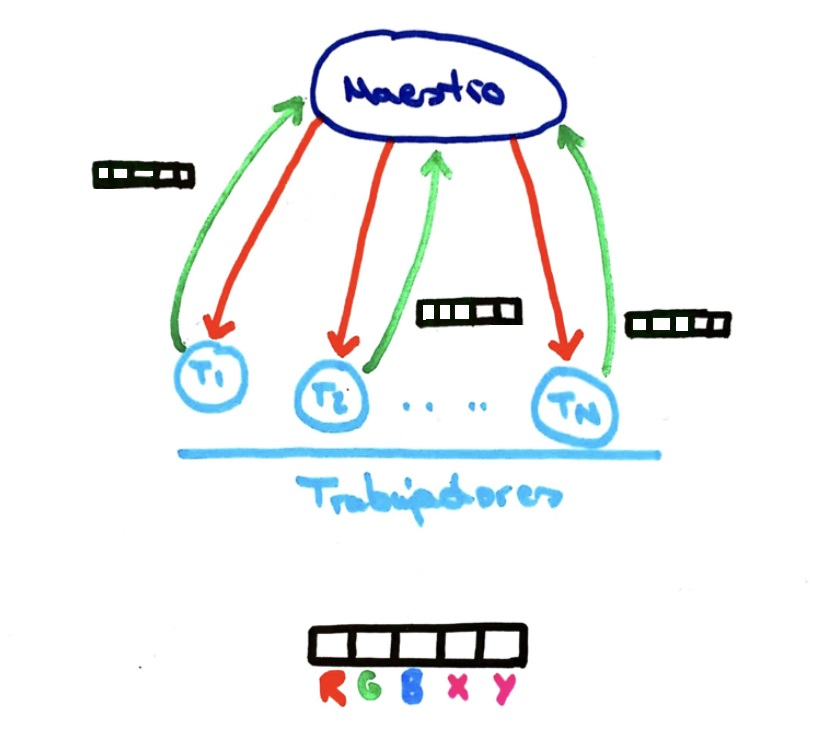
\includegraphics[width=120mm]{flujo.PNG}
\caption{Representación del flujo de eventos.}
\label{fig:flujo}
\end{figure}




\newpage
\section{Diseño de la solución}
En este apartado se describirá las funciones que componen el programa, el cual, hace posible el funcionamiento del proceso anteriormente descrito.

\subsection{Función principal del programa (\textit{main})}
Esta es la función principal del programa, en la cual como se puede observar lo primero que se lleva a cabo es la definición de las variables a utilizar, como: \textit{rank}, \textit{size}, \textit{error-codes} (vector donde se almacenarán si surge algún error a la hora de crear los trabajadores), \textit{commPadre} (comunicador del proceso padre, utilizado a la hora de enviar y recibir información entre los procesos), status (indica el estado de la recepción de datos por parte del proceso padre), etc.

Como se puede observar en esta función principal (\textit{main}), encontramos dos bifurcaciones, las cuales pertenece la primera al flujo de eventos del proceso \textbf{maestro} (Rank 0), y la otra bifurcación que pertenece a las acciones que debe de llevar a cabo los \textbf{trabajadores} (demás ranks).


Tras esto se declarán las primitivas de \textit{\textbf{MPI}} como: 
\begin{itemize}
	\item \textit{MPI-Init}() \cite{transpas}: Para inicializar la estructura de comunicación de MPI entre los procesos. 
	\item \textit{MPI-Comm-Size}() \cite{transpas}: Para obtener el tamaño de la comunicacion (número de proceso a ejecutar en este caso, ranks), etc.
	\item \textit{MPI-Comm-rank}() \cite{transpas}: Para establecer el identificador de cada proceso \textit{rank}.
	\item \textit{MPI-Comm-get-parent}() \cite{org}: Se encarga de retornar el comunicador del proceso padre al proceso actual.
\end{itemize}

También en esta función se llevan a cabo las llamadas a las demás tipos de funciones que componen el programa
\lstinputlisting[language=C]{code/main.c}


\subsection{Recepción de los píxeles (\textit{receive-points})}
El encargado de ejecutar esta función (como bien hemos dicho anteriormente) es el proceso \textbf{maestro} (Rank 0). La cual, se encarga de invocar a la primitiva de MPI \cite{org}, \textbf{\textit{MPI-Recv}}() \cite{org}, para la recepción por medio de un buffer de tipo entero (point-to-paint), en el cual se almacenará los datos del mensaje enviado por un trabajador, este contiene la información necesaria para pintar ese píxel en la imagen, tras esto se pinta dicho píxel por pantalla con la función \textit{\textbf{dibujarPunto()}}.
\lstinputlisting[language=C]{code/receive_points.c}


\subsection{Calcular líneas del fichero (\textit{calculate-file-lines})}
Esta función llevada a cabo por todo proceso de tipo trabajador (distinto de Rank 0), se encarga de calcular la zona de trabajo que le corresponde a cada trabajador (líneas que le corresponden). Se realiza como se puede observar por la division entre \textit{IMAGE-SIDE} (lado de la imagen), que es el número de filas o líneas que tiene la imagen (400 en este caso), entre el \textit{EMPLOYEES-NUMBER} (constante que representa el número de trabajadores). También calculamos el resto de la operación anterior, y el número de bytes de cada fila (\textit{row-bytes}), esta variable almacenara el número de bytes o elementos por fila.
\lstinputlisting[language=C]{code/calculate_file_lines.c}


\subsection{Asignar zona de trabajo (\textit{assign-work-zone})}
El encargado de ejecutar esta función al igual que la anterior, y las posteriores es todo proceso de tipo trabajador (distinto a Rank 0). Esta función de asignar su zona de trabajo a cada proceso trabajador. Es decir, de asignarle una linea de inicio y otra de fin. Para ello cada \textbf{línea de comienzo} (\textit{start-line}) de cada trabajador será: su \textit{rank} x \textit{lines-per-employee} (cantidad de líneas asignada a cada trabajador). Tras esto se calculará la linea de fin (\textit{end-line}), que se obtendrá de calcular la misma operación anterior pero incrementando el rank en 1. En cambio, si el rank actual es el último, en este caso se le asignará también \textit{rest-lines} (resto de las líneas si es que las hubiese).
\lstinputlisting[language=C]{code/assign_work_zone.c}


\subsection{Apertura del fichero (\textit{open-file})}
En esta función llevada a cabo por cada trabajador, se realiza la apertura del fichero de la imagen. Para ello como se puede observar se utiliza la función \textit{\textbf{MPI-File-open()}} \cite{org}, y posteriormente se utiliza la función \textbf{\textit{MPI-File-set-view()}} \cite{org} la cual posiciona a cada rank en su zona de trabajo, y evitar así que interfieran entre ellos.\\
Finalmente devolvemos el descriptor del archivo, ya que sera necesario más adelante. 
\lstinputlisting[language=C]{code/open_file.c}


\subsection{Leer un píxel de la imagen (\textit{read-pixel})}
En esta función llevada a cabo por cada trabajador, donde leerá y almacena la información de cada píxel de la imagen (que pertenezca a su zona de trabajo), mediante la función \textit{\textbf{MPI-File-read()}} \cite{org}. Esta información se almacenara en un vector de tipo \textit{unsigned char} denominado \textit{\textbf{píxel}}. Donde se almacenarán los valores de ese pixel correspondientes a cada color primario, es decir, \textbf{R, G, B} (Rojo, Verde y Azul).
Tras esto, se llamará ma la función aplicar filtro (\textbf{\textit{apply-filter}}()).
\lstinputlisting[language=C]{code/read_pixel.c}


\subsection{Comprobación del píxel (\textit{check-pixel})}
En esta función llevada a cabo por cada trabajador, se comprobará si el valor de los colores primarios que forman el píxel, se encuentra dentro de su rango, ya que el color se calcula entre el rango de 0 a 255.
\lstinputlisting[language=C]{code/check_pixel.c} 


\subsection{Aplicar filtro (\textit{apply-filter})}
En esta función llevada a cabo por cada trabajador, una vez que tiene la información del pixel leido (almacenada en \textbf{\textit{pixel}}), se asignará dicha información, junto con la posición en la que se encentra el pixel en la imagen (Fila, Columna), al vector de tipo entero \textit{\textbf{point-to-paint}}. Este será utilizado para almacenar la información del píxel durante su configuración, es decir, para aplicarle el filtro que haya deseado el usuario.

Los filtros de los cuales dispone el programa, como se puede observar, son:
\begin{itemize}
	\item \textbf{Por defecto}: Color que tiene el píxel en la imagen original.
	\item \textbf{Sepia.}
	\item \textbf{Blanco y Negro.}
	\item \textbf{Negativo}: color complementario al que se encuentre el píxel.
\end{itemize}

Una vez, que se ha aplicado el filtro, se debera de comprobar si el filtro ha sido aplicado de forma correcta, mediante la función \textit{\textbf{check-pixel}}.\\
Finalmente, se mandará la información correspondiente al pixel (almacenda en \textit{\textbf{point-to-paint}})al proceso maestro, mediante la función \textbf{\textit{MPI-Send()}} \cite{org}, para que así el maestro pueda pintar el píxel por pantalla.
\lstinputlisting[language=C]{code/apply_filter.c}


%%%%%%%%%%%%%%%%%%%%%%%%%%%%%%%%%%%%%%%%%%%%%%%%%%%%%%%%%%%%%%%%%%%%%%%%%%%%%%%%
%%%%%%%%% 						BIBLIOGRAFIA 						   %%%%%%%%%
%%%%%%%%%%%%%%%%%%%%%%%%%%%%%%%%%%%%%%%%%%%%%%%%%%%%%%%%%%%%%%%%%%%%%%%%%%%%%%%%
\newpage
\bibliography{biblist}
\bibliographystyle{plain}

%\nocite{*} Permite citar todas las referencias en el archivo .bib

% Añadir la bibliografía al Índice de contenidos
\ifspanish
	\addcontentsline{toc}{section}{Referencias}
\else
	\addcontentsline{toc}{section}{References}
\fi




\end{document}
